% Five-drone scenario: cable 1 snaps at t=7.0s, cable 3 snaps at t=12.0s
% Three panels: pre-fault (t=6.0), after first fault (t=8.0), settled after both (t=15.0)
% XY-plane relative positions (drone - load)
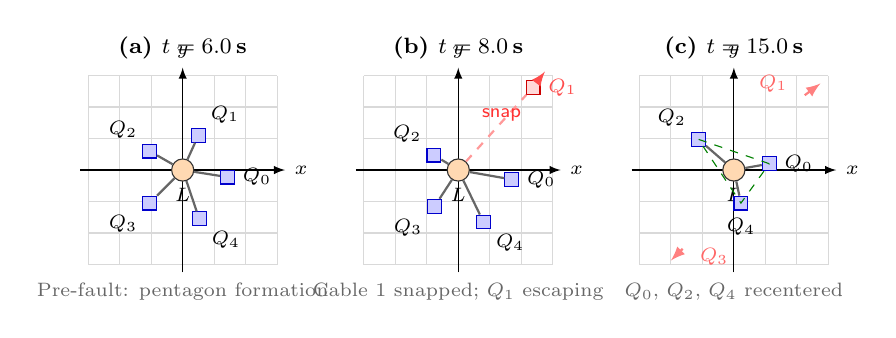
\begin{tikzpicture}[
  drone/.style={draw=blue!80!black, fill=blue!20, minimum size=5pt, inner sep=0pt, font=\tiny},
  faulted/.style={draw=red!80!black, fill=red!15, minimum size=5pt, inner sep=0pt, font=\tiny},
  escaped/.style={draw=red!60, fill=red!5, minimum size=5pt, inner sep=0pt, dashed, font=\tiny},
  payload/.style={circle, draw=black!80, fill=orange!30, minimum size=8pt, inner sep=0pt},
  cable/.style={thick, black!60},
  snapped/.style={thick, red!40, dashed},
  panel/.style={font=\footnotesize\bfseries},
  lbl/.style={font=\scriptsize},
  >=latex
]

% === Panel (a): t = 6.0 s — Pre-fault ===
\begin{scope}[shift={(0,0)}]
  \draw[gray!30, thin] (-1.2,-1.2) grid[step=0.4] (1.2,1.2);
  \draw[->] (-1.3,0) -- (1.3,0) node[right, font=\scriptsize]{$x$};
  \draw[->] (0,-1.3) -- (0,1.3) node[above, font=\scriptsize]{$y$};

  % Payload at origin
  \node[payload] (L) at (0,0) {};
  \node[lbl, below=3pt] at (L) {$L$};

  % Drone positions relative to load at t=6.0
  % drone0-load: (2.579-2.011, 1.001-1.091) = (0.568, -0.090)
  % drone1-load: (2.207-2.011, 1.527-1.091) = (0.196, 0.436)
  % drone2-load: (1.592-2.011, 1.330-1.091) = (-0.419, 0.239)
  % drone3-load: (1.595-2.011, 0.671-1.091) = (-0.416, -0.420)
  % drone4-load: (2.217-2.011, 0.470-1.091) = (0.206, -0.621)
  \node[drone] (D0) at (0.57, -0.09) {};
  \node[drone] (D1) at (0.20,  0.44) {};
  \node[drone] (D2) at (-0.42, 0.24) {};
  \node[drone] (D3) at (-0.42,-0.42) {};
  \node[drone] (D4) at (0.21, -0.62) {};

  % Cables
  \draw[cable] (L) -- (D0);
  \draw[cable] (L) -- (D1);
  \draw[cable] (L) -- (D2);
  \draw[cable] (L) -- (D3);
  \draw[cable] (L) -- (D4);

  % Labels
  \node[lbl, right=2pt] at (D0) {$Q_0$};
  \node[lbl, above right=1pt] at (D1) {$Q_1$};
  \node[lbl, above left=1pt] at (D2) {$Q_2$};
  \node[lbl, below left=1pt] at (D3) {$Q_3$};
  \node[lbl, below right=1pt] at (D4) {$Q_4$};

  \node[panel] at (0, 1.55) {(a) $t = 6.0$\,s};
  \node[lbl, text=black!60] at (0, -1.55) {Pre-fault: pentagon formation};
\end{scope}

% === Panel (b): t = 8.0 s — 1 s after first fault (cable 1) ===
\begin{scope}[shift={(3.5,0)}]
  \draw[gray!30, thin] (-1.2,-1.2) grid[step=0.4] (1.2,1.2);
  \draw[->] (-1.3,0) -- (1.3,0) node[right, font=\scriptsize]{$x$};
  \draw[->] (0,-1.3) -- (0,1.3) node[above, font=\scriptsize]{$y$};

  % Payload at origin
  \node[payload] (L) at (0,0) {};
  \node[lbl, below=3pt] at (L) {$L$};

  % Drone positions relative to load at t=8.0
  % drone0-load: (3.150-2.468, 0.941-1.065) = (0.682, -0.124)
  % drone1-load: (3.566-2.468, 3.303-1.065) = (1.098, 2.238) -- escaping, off scale
  % drone2-load: (2.161-2.468, 1.251-1.065) = (-0.307, 0.186)
  % drone3-load: (2.168-2.468, 0.601-1.065) = (-0.300, -0.464)
  % drone4-load: (2.783-2.468, 0.403-1.065) = (0.315, -0.662)
  \node[drone] (D0) at (0.68, -0.12) {};
  \node[drone] (D2) at (-0.31, 0.19) {};
  \node[drone] (D3) at (-0.30,-0.46) {};
  \node[drone] (D4) at (0.32, -0.66) {};

  % D1 escaping -- show at edge with arrow
  \node[faulted] (D1) at (0.95, 1.05) {};
  \draw[->, red!70, thick] (D1) -- ++(0.15, 0.2);

  % Cables
  \draw[cable] (L) -- (D0);
  \draw[snapped] (L) -- (D1);
  \draw[cable] (L) -- (D2);
  \draw[cable] (L) -- (D3);
  \draw[cable] (L) -- (D4);

  % Snap marker
  \node[font=\scriptsize, red!80] at (0.55, 0.70) {\textsf{snap}};

  % Labels
  \node[lbl, right=2pt] at (D0) {$Q_0$};
  \node[lbl, right=2pt, red!70] at (D1) {$Q_1$};
  \node[lbl, above left=1pt] at (D2) {$Q_2$};
  \node[lbl, below left=1pt] at (D3) {$Q_3$};
  \node[lbl, below right=1pt] at (D4) {$Q_4$};

  \node[panel] at (0, 1.55) {(b) $t = 8.0$\,s};
  \node[lbl, text=black!60] at (0, -1.55) {Cable 1 snapped; $Q_1$ escaping};
\end{scope}

% === Panel (c): t = 15.0 s — Settled after both faults ===
\begin{scope}[shift={(7.0,0)}]
  \draw[gray!30, thin] (-1.2,-1.2) grid[step=0.4] (1.2,1.2);
  \draw[->] (-1.3,0) -- (1.3,0) node[right, font=\scriptsize]{$x$};
  \draw[->] (0,-1.3) -- (0,1.3) node[above, font=\scriptsize]{$y$};

  % Payload at origin
  \node[payload] (L) at (0,0) {};
  \node[lbl, below=3pt] at (L) {$L$};

  % Drone positions relative to load at t=15.0
  % drone0-load: (0.318-(-0.134), 0.035-(-0.043)) = (0.452, 0.078)
  % drone1: escaped far (5.1, 6.3) -- off screen
  % drone2-load: (-0.579-(-0.134), 0.347-(-0.043)) = (-0.445, 0.390)
  % drone3: escaped far (-1.8, -5.8) -- off screen
  % drone4-load: (-0.041-(-0.134), -0.464-(-0.043)) = (0.093, -0.421)
  \node[drone] (D0) at (0.45, 0.08) {};
  \node[drone] (D2) at (-0.45, 0.39) {};
  \node[drone] (D4) at (0.09, -0.42) {};

  % Cables to surviving drones
  \draw[cable] (L) -- (D0);
  \draw[cable] (L) -- (D2);
  \draw[cable] (L) -- (D4);

  % Off-screen escaped drones
  \draw[->, red!50, thick, dashed] (0.90, 0.95) -- (1.10, 1.10);
  \node[lbl, red!60] at (0.50, 1.10) {$Q_1$};
  \draw[->, red!50, thick, dashed] (-0.65, -1.00) -- (-0.80, -1.15);
  \node[lbl, red!60] at (-0.25, -1.10) {$Q_3$};

  % Labels
  \node[lbl, right=2pt] at (D0) {$Q_0$};
  \node[lbl, above left=1pt] at (D2) {$Q_2$};
  \node[lbl, below=2pt] at (D4) {$Q_4$};

  % Triangle annotation
  \draw[green!50!black, thin, dashed] (D0.center) -- (D2.center) -- (D4.center) -- cycle;

  \node[panel] at (0, 1.55) {(c) $t = 15.0$\,s};
  \node[lbl, text=black!60] at (0, -1.55) {$Q_0$, $Q_2$, $Q_4$ recentered};
\end{scope}

\end{tikzpicture}
